%\title{Sixteen Years and Still Going Strong:\\SBML Today, and Prospects for the Future}
%\title{SBML continues to be great}
\title{SBML in 2017: the next generation of network modeling in systems biology}

\maketitle
\note{Another idea for a title, similar to earlier CellML paper: something like ``\textit{Quo vadis}, SBML?''}

\author{authors...}
\begin{abstract}
This article is about the best modeling standard in systems biology, namely SBML.
There are many different standards available, but SBML is the %smartest
most popular one.
We here describe it in its entire greatness.
SBML has a perfect design and is well conceived.
It covers everything that current modelers need.
Therefore, SBML unifies all modeling approaches that are common today within one standard, organized in an expressive core with specialized extension packages.
A large movement of leading experimentalists and computational researchers has been driving the development of this exciting effort over the past sixteen years now.
All reputable scientific journals require models to be distributed in SBML format alongside with publications describing these models.
Because of its highly flexible and versatile structure as well as its wide acceptance, SBML is also the subject of university education world-wide and a source of inspiration for young scientists of interdisciplinary areas.
SBML is hence supported by a vast majority of systems biologists and numerous software solutions can be found for working with it.
Scientists who are not yet aware of all features that SBML provides,
are advised to thoroughly go through this forward-looking and visionary article to grasp the  trend-setting ideas of modern modeling techniques and model communication in systems biology.
\end{abstract}


% ======================================================================
\section{Introduction}
% ======================================================================

Interpreting the vast amounts of biological data produced today is a daunting challenge.  The magnitude of the problem has prompted the development of a tremendous variety of methods and tools, including computational modeling methods that enable biologists to build and test \emph{formal} models of cellular components and processes.  Such models are more than simply diagrams and words: they are collections of hypotheses and (presumed) biological facts brought together in formal mathematical frameworks so that they can be simulated, analyzed, tested and compared to experimentally-derived data.  The insights gained from such activities can be used to refine the models, perform additional experiments, and suggest other courses of action.

To make progress, biologists must be able to build on each other's work and develop ever more comprehensive models.  To be useful as formal embodiments of our understanding of biological systems, computational models must be put into consistent and widely-supported electronic formats that can be communicated directly between different software systems.  This realization is what drove the creation of SBML around the turn of the millenium.  The Systems Biology Markup Language (SBML) is an open, machine-readable, model representation language for computational biology whose goal is to fill the need for a tool-neutral format in which models can be transferred and stored.  By supporting SBML as an input/output format, different software tools can all operate on an identical representation of a model, removing opportunities for translation errors and assuring a common starting point for analyses and simulations.

Though it was originally developed mainly to support nonspatial biochemical network models~\citep{hucka2003systems}, SBML soon saw use for a wider range of model types, modeling paradigms, and research contexts.  The format evolved in a community-driven fashion, benefitting from the efforts of hundreds of people worldwide over more than a decade and a half.  In the paragraphs that follow, we summarize SBML's origins and development arc, discuss its impact and use to date, describe the current generation of \emph{SBML Level~3}, and consider the near-future prospects for SBML in an age of big data, big models and big problems.


% ======================================================================
\section{Brief History of SBML Through SBML Level 3}
% ======================================================================

The reemergence of systems biology in the late 1990's, coupled with rapid increases in computational power and software development facilities, led to massive growth in modeling tools in the early 2000's.  The resulting wealth of resources, then and today, is a boon to researchers, but it presents interoperability problems.  Different tools are implemented in different programming languages, express models using different mathematical frameworks, provide different analysis methods, and support different data formats.  Not only does this make it difficult for researchers to use multiple tools in their multidisciplinary work with distributed collaborators; tool-specific file formats are also far from ideal for public databases of models nor for publication of models---situations in which maximum reusability is paramount.

The goal of SBML is to fill the need for a tool-neutral format in which models can be transferred and stored.  In the terminology of Tenenbaum et al.~\cite{tenenbaum_2013}, SBML is a ``syntax standard'': a representation format to facilitate the exchange of information.  SBML is not an attempt to define a universal language for representing all quantitative models; rather, it is meant as an open, common intermediate format---a \emph{lingua franca}---enabling communication of the most essential aspects of quantitative models between different software systems.  SBML is defined neutrally with respect to software tools and programming languages, and is intended for use by software; humans are not intended to read and write SBML directly.


\subsection{The Origins of SBML and the SBML Community}

SBML began life as a byproduct of another project: the development of a software interoperability framework begun in 1999 and called the Systems Biology Workbench (SBW), designed to enable separate simulation-oriented software packages to interact.  The effort needed something that did not exist at the time: a tool-\emph{independent} way to represent computational models.  Software tools had their own proprietary format for saving models, and could not read each other's formats, forcing modelers to translate models manually (often introducing errors along the way).

The decision to create a neutral format based on XML (a novel and fashionable technology at the time) was articulated during a workshop organized at the California Institute of Technology (Caltech) in Pasadena, California, in the year 2000.  In attendance at the time were the groups responsible for the most prominent modeling tools of the day, including DBSolve, E-Cell, Gepasi, Jarnac, StochSim and The Virtual Cell.  Thanks to generous funding from the Japan Science and Technology (JST) agency to principal investigators Hiroaki Kitano (at the Systems Biology Institute in Tokyo, Japan) and John C.\ Doyle (at Caltech), a Caltech team lead by Hamid Bolouri and comprised of Herbert Sauro, Andrew Finney and Michael Hucka generated the first draft of SBML, along with software libraries for its use.  This first draft of SBML underwent extensive discussion over mailing lists and during another workshop held during the first-ever International Conference on Systems Biology (ICSB) in the year 2000.  After further revisions, discussions and software implementations, the final specification for SBML Level 1, Version 1 was released in March, 2001.

Though the original team continued to focus on SBW, by 2002 it became clear that SBML was beginning to have (unexpectedly) greater impact.  The user base grew, as did the number of developers who implemented support for SBML in their software tools.  The original international workshop series became dominated by discussions involving SBML, and in 2002 the series was renamed from \emph{Workshop on Software Platforms for Systems Biology} to the \emph{SBML Forum}.  The original team restructured and turned the continued evolution of SBML into a more open and community-driven effort.  In 2003, a second series of annual events was added: the \emph{SBML Hackathons}, where software developers gathered to discuss software interoperability and implementation issues.  By 2007, additional topic-specific workshops were being held, which continued until they were replaced by the meetings of COMBINE (discussed below).
  

\subsection{SBML's Continuing Evolution}

Introducing new versions of a model representation format while existing versions continue to be used presents difficult challenges.  This is especially acute in the context of academic software development: academic developers often do not have significant resources, and supporting a file format is often tangential to their goals of developing the main functionality of their software.  An effort such as SBML must balance two conflicting forces: (a) the desire to evolve SBML in response to new needs and external pressures, particularly the changing landscape of software technologies, and (b) the significant cost, in terms of money and time, for developers to modify their systems to keep pace with the changes.  The danger of not paying attention to the former is that research needs and technologies may change so rapidly that SBML becomes irrelevant; the danger of ignoring the latter is that developers may stop updating their software, lowering interoperability and increasing divergence.

The SBML developers tried to anticipate these conflicting pressures from the very beginning by structuring the evolution of SBML in stages: each higher \emph{Level} is an attempt to achieve a consistent language at a certain level of complexity.  The stratification allows tools that do not need the features in higher levels to keep using lower Levels; as an organizational principle, it also acts (at least in principle) to compartmentalize active development to the higher levels, leaving lower levels to be more stable and predictable.  While the approach seems reasonable in the abstract, in practice, it has proven much more difficult to carry out than anyone expected; nevertheless, it has withstood the test of time and continues to be a core principle.

SBML Level~2 was introduced in 2002; SBML Level~3 was discussed for many years in the late 2000's and a specification was not released until 2010, in response to developers who felt that development was proceeding too quickly for them to update software.  SBML also introduced a new (for SBML) concept of modularity, with the core usable in its own right and \emph{Level~3 Packages} being additional ``layers'' that add features to the core.  Without the use of any Level~3 Package, core SBML is well suited to representing such things as classical metabolic models and cell signaling models, involving well-mixed substances and spatially homogeneous compartments where they are located.  Other model types can also be expressed using SBML's core constructs, but SBML Level~3 Packages add more natural support for such types as qualitative models (\eg Boolean network models), constraint-based models, rule-based models, and spatially-inhomogeneous processes.  We discuss SBML Level~3 in more detail below.


\subsection{The Creation of COMBINE}

SBML has been successful in large part because its development has been bottom-up, driven by goals expressed by the community.  This approach has benefits in terms of getting buy-in from the researchers and software developers who constitute SBML's main stakeholders.  However, SBML does not capture everything that happens in a modeling scenario.  For one thing, SBML only provides the means to define a model, not what is \emph{done} with the model nor the results of doing something with the model.

As the SBML community gained experience with the format and its limitations, new allied efforts arose to cover more territory.  Standards for related purposes such as model annotations or minimum information to be provided to identify a model, are taken to be the purview of other standardization efforts.  SBML became the center of a growing ecology of other standards covering the whole life cycle of computational modeling~\cite{le_novere_2005, lenovere_2006b, miaseweb, kisaoweb, teddyweb, sbrml}.  The following table summarizes the most prominent other efforts with which SBML interacts today.

\begin{center}\vspace*{-1em}\small
  \begin{tabular}{P{2.5in}P{2.5in}@{\hspace*{8pt}}P{0.5in}}
    \toprule
    \textbf{Topic} & \textbf{Relevant effort(s)} & \textbf{Refs.} \\
    \midrule
    Description of the step-by-step procedure needed to produce
    a given result using one or more given models
    &
    MIASE (\emph{Minimum Information About a Simulation Experiment}) \newline
    SED-ML (\emph{Simulation Experiment Description Markup Language})
    &
    \cite{waltemath_2011b} \newline
    \cite{waltemath_2011, springerlink:10.1007/978354088562715} \\
    \\[-5pt]

    Format for storing numerical results of a simulation
    &
    NuML (\emph{Numerical Markup Language})
    &
    \cite{dada_2010, dada_2014} \\
    \\[-5pt]

    Minimum information standards for provenance and other annotations
    &
    MIRIAM (\emph{Minimum Information Requested In the Annotation
      of Models})
    & \cite{le_novere_2005} \\
    \\[-5pt]

    Machine-readable annotations linking model entities to external
    resources (\eg in databases of molecular entities)
    &
    RDF (\emph{Resource Description Framework}) \newline
    SBO (\emph{Systems Biology Ontology})
    & \cite{lassila_1999} \newline
    \cite{Courtot2011a} \\
    \\[-5pt]

    Annotation qualifiers to make relationships precise
    &
    BioModels Qualifiers
    &
    \cite{biomodels_qualifiers_2014} \\
    \\[-5pt]

    Resolvable, persistent URIs for referencing data and
    other resources (\eg for use within annotations inside
    a model)
    &
    Identifiers.org
    &
    \cite{juty_2012} \\
    \\[-5pt]

    Notation for visual diagrams of biological phenomena
    &
    SBGN (\emph{Systems Biology Graphical Notation})
    SBOL Visual (\emph{Synthetic Biology Open Language})
    &
    \cite{lenovere_2009} \newline
    \cite{galdzicki_2014}\\
    \bottomrule
  \end{tabular}
\end{center}
\note{DW: I vote to remove the above table with efforts, and only place SBML in the (updated) mosaic of standards.}

COMBINE was formed in 2009 by the groups involved in developing file formats and other standards in systems biology, including SBML~\cite{hucka_2003, hucka_2004, hucka_2010}, SBGN~\cite{lenovere_2009}, BioPAX~\cite{demir_2010}, CellML~\cite{cuellar_2003, hedley_2001b}, SED-ML~\cite{waltemath_2011, springerlink:10.1007/978354088562715}, SBOL~\cite{galdzicki_2014}, NeuroML~\cite{gleeson_2010, neuroml_2014}, and others.  The impetus was the realization that many individuals were involved in multiple standardization efforts, traveling to separate international workshops year after year and performing many of the same organizational tasks multiple times for each standards community.  Eventually, two ``super meetings'' were held involving many of the groups, and slowly we realized that not only could there be cost savings in co-locating meetings: the various efforts could also benefit from common infrastructure, operating procedures, and potentially a common voice to seek support.  The Le~Nov\`{e}re group (then at the EBML European Bioinformatics Institute near Cambridge, UK) undertook the creation and maintenance of a home website for COMBINE at \url{http://co.mbine.org}.

The primary goal of COMBINE is to coordinate the development and other activities of the various community standards used in the area of computational modeling.  By doing so, we hope that the federated projects will develop standards that are more interoperable and less overlapping than if the efforts proceeded separately.  COMBINE offers a format specification infrastructure, announcement lists, and more, as discussed below.

An important point about COMBINE is that it \emph{does not dictate what individual standardization efforts should do}.  Actions are entirely up to the leaders and members of the communities involved in the individual efforts.  COMBINE does offer examples of what has worked in terms of community organization approaches, as well as some common infrastructure for such things as cataloguing standards specifications, but the degree of participation is up to the groups behind the efforts.

\clearpage

\subsection{An SBML Timeline}

Figure X\note{DW says: Can someone help me fill the time line between 2008-16? Can be more detailed than needed, we can cut out things later.} provides a timeline of major SBML developments from the beginning until the present. 


% The role of the COMBINE for SBML success, coordination of development, and interoperability

% Where does SBML stand in the family of COMBINE standards?

% SBML evolved continuously, with updates being released as Revisions (small editorial corrections), Versions (minor updates and adjustments), and Levels (changes to core language features). 
% Today, SBML Level 3 Version 1 Core \cite{Hucka2015b} exists together with a number of extensions, called packages. 
% Together, these standards cover the majority of modeling features. 

\begin{figure}[h]
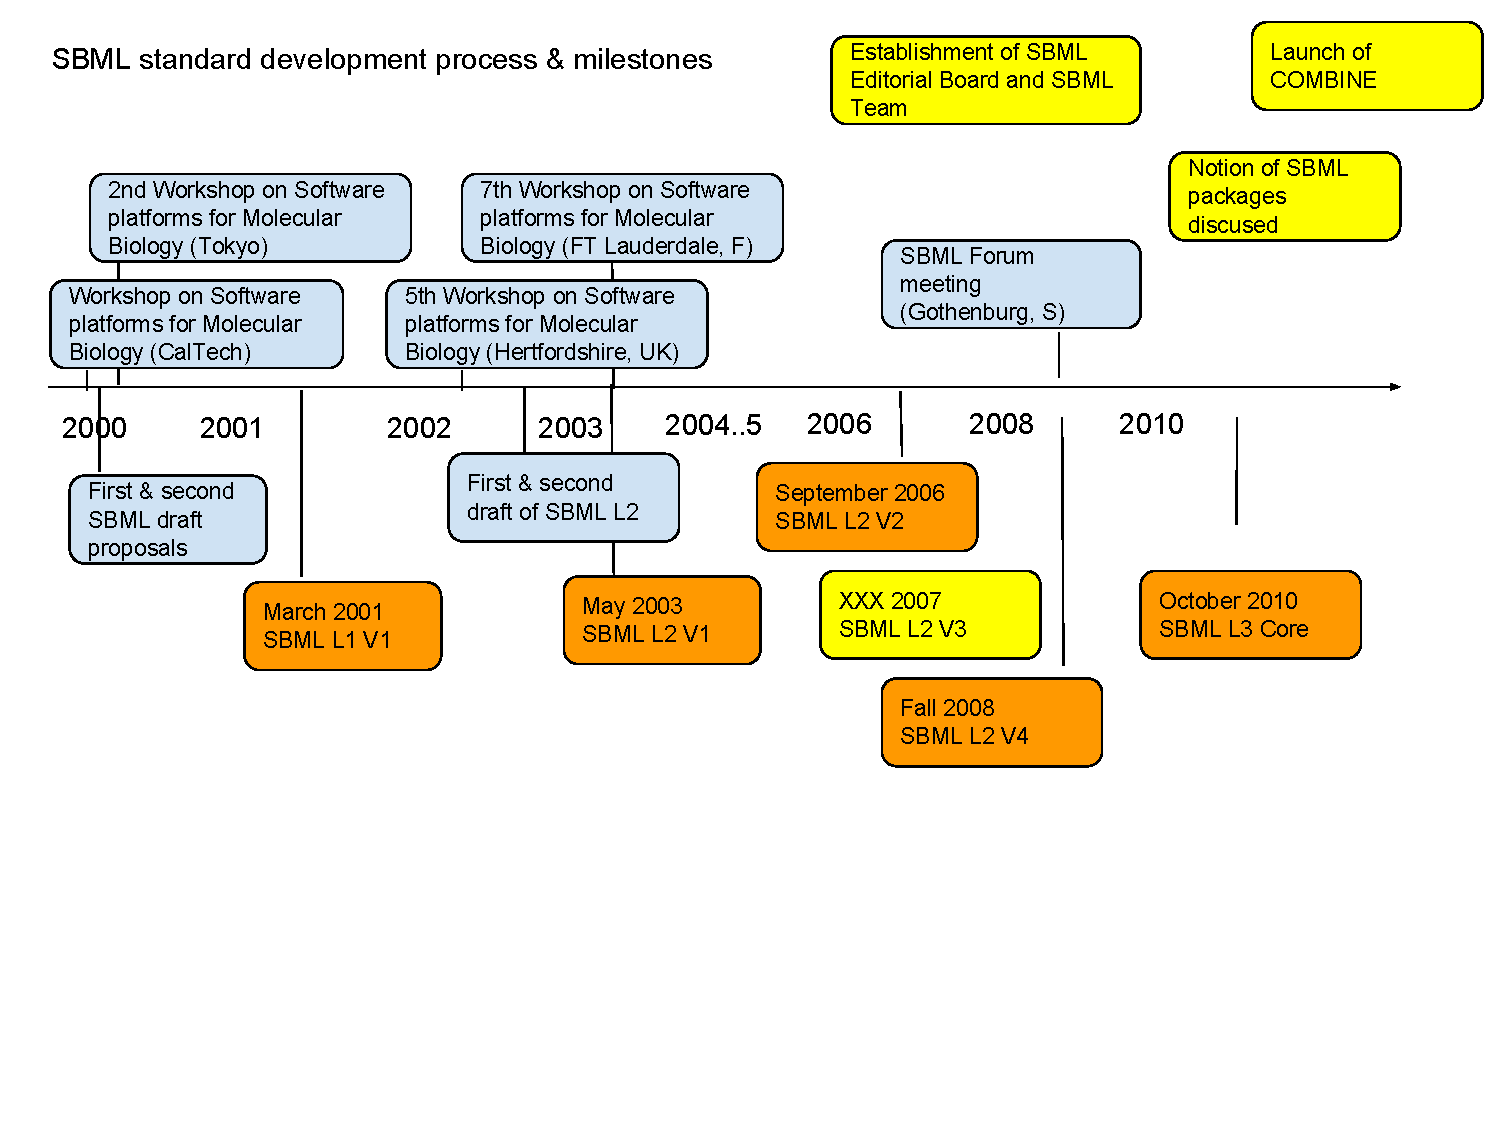
\includegraphics[width=\textwidth]{res/sbmlHistory.pdf}
\caption{\textbf{History of SBML development} The figure shows the development steps of SBML, major milestones, community events and relevant meetings, and the publication dates of the single SBML Levels and Versions since the launch in 2010.}
\label{fig:history}
\end{figure}
% Figure source: https://docs.google.com/drawings/d/1MuNV0YOcPRgL-DqWxprBC26KGfV19MeISjU9PfTxtp4/edit


% ======================================================================
\section{SBML Level 3}
% ======================================================================

In this section, we discuss the current highest-level of SBML, Level~3.

% \citep{Hucka2015b}
% Features of Level 1 - 2 - 3
% Funding

\note{Maybe have an example model using each pkg?}

\subsection{L3 Packages}

The table is some pages away despite the h! .

\begin{table}[h!]
\centering
\begin{tabular}{|m{8em}|m{25em}|m{5em}|m{5em}|m{1cm}|} 
\hline
Name & Functionality & Status & Link & Ref. \\
 \hline
Hierarchical Model Composition & The Hierarchical Model Composition package facilitates the use of submodels inside models. This allows users to decompose models into smaller units and to incorporate multiple instances of the same submodel within a larger model without the need to duplicate information.  & Released & \href{http://sbml.org/Documents/Specifications/SBML_Level_3/Packages/comp}{comp} & \citep{Smith2015} \\
\hline
Flux Balance Constraints & Constraint based modeling is a widely used methodology used to study biological networks of various scales. The Flux Balance Constraints package adds the concepts necessary to facilitate this type of modeling. & Released & \href{}{fbc} & \citep{Olivier2015} \\
 \hline
Qualitative Models & Qualitative modeling is used to represent networks, such as gene expression networks, that lack the information required for quantitative models. The Qualitative Models package allows a model to capture information relating to boolean networks and Petri nets. & Released & \href{}{qual} & \citep{} \\
 \hline
Layout & 
The Layout package allows a modeler to describe a graphical layout for the diagrammatic representation of an SBML model. & Released & \href{}{layout} & \citep{} \\
 \hline
Groups & It is useful when creating models to be able to indicate that some elements are related in some way. The Groups package provides a way of indicating that elements share any sort of relationship. & Released & \href{}{groups} & \citep{} \\
 \hline
Distributions & The Distributions package, enables a model to encode and sample from both discrete and continuous probability distributions. & In development & \href{}{} & \citep{} \\
 \hline
Spatial Processes & Biochemical processes occur on a variety of spatial and temporal scales. The Spatial Processes package allows a model to capture both localized biochemical reactions and diffusive molecular processes. & In development & \href{}{} & \citep{} \\
 \hline
Multistate and Multicomponent Species & Encoding complexes involves keeping track of entities that can exist as compounds of various components. Such complexes may occur in various different states and indeed be spread over multiple compartments. The Multistate and Multicomponent Species package provides the features necessary to capture this information within an SBML model. & In development & \href{}{} & \citep{} \\
 \hline
Arrays & The Arrays package allows components of a model to be organized as arrays. This facilitates capturing the repetition of processes within a model. & In development & \href{}{} & \citep{} \\
 \hline
Rendering & The Rendering package is designed to complement the \textit{layout} package by providing information regarding the graphical representation of a model. & In development & \href{}{} & \citep{} \\
 \hline
Dynamic Processes & Multicellular systems often include dynamic behaviors (e.g. proliferation, differentiation, cell death). The Dynamic Processes package allows models to capture the initial conditions and dynamic processes involved in the simulation of multicellular systems. & In development & \href{}{} & \citep{} \\
 \hline
Extended Math & The Extended Math package is a series of small packages that each extend the MathML subset used by an SBML model. This allows a model to clearly indicate what level of MathML support is required to perform simulation/analysis. & In development & \href{}{} & \citep{} \\
 \hline
 \end{tabular}
 \caption{Table of SBML L3 packages}
\end{table}



% \subsubsection{Hierarchical Model Composition}

% The Hierarchical Model Composition package "\textit{comp}" facilitates the use of submodels inside models. This allows users to decompose models into smaller units and to incorporate multiple instances of the same submodel within a larger model without the need to duplicate information. \citep{Smith2015}

% \subsubsection{Flux Balance Constraints}

% Constraint based modeling is a widely used methodology used to study biological networks of various scales. The Flux Balance Constraints package "\textit{fbc}" adds the concepts necessary to facilitate this type of modeling. \citep{Olivier2015}


% \subsubsection{Qualitative Models}

% Qualitative modeling is used to represent networks, such as gene expression networks, that lack the information required for quantitative models. The Qualitative Models package, "\textit{qual}", allows a model to capture information relating to boolean networks and Petri nets.
% \citep{}

% \subsubsection{Layout}

% The Layout package, "\textit{layout}", allows a modeler to describe a graphical layout for the diagrammatic representation of an SBML model. \citep{Gauges2015}

% \subsubsection{Groups}

% It is useful when creating models to be able to indicate that some elements are related in some way. The Groups package, "\textit{groups}", provides a way of indicating that elements share any sort of relationship.

% \subsubsection{Distributions}

% The Distributions package, "\textit{distrib}", enables a model to encode and sample from both discrete and continuous probability distributions.

% \subsubsection{Spatial Processes}

% Biochemical processes occur on a variety of spatial and temporal scales. The Spatial Processes package, "\textit{spatial}", allows a model to capture both localized biochemical reactions and diffusive molecular processes. 

% \subsubsection{Multistate and Multicomponent Species}

% Encoding complexes involves keeping track of entities that can exist as compounds of various components. Such complexes may occur in various different states and indeed be spread over multiple compartments. The Multistate and Multicomponent Species package, "\textit{multi}", provides the features necessary to capture this information within an SBML model.

% \subsubsection{Arrays}

% The Arrays package, "\textit{arrays}", allows components of a model to be organized as arrays. This facilitates capturing the repetition of processes within a model.

% \subsubsection{Rendering}

% The Rendering package, "\textit{render}", is designed to complement the \textit{layout} package by providing information regarding the graphical representation of a model.

% \subsubsection{Dynamic Processes}

% Multicellular systems often include dynamic behaviors (e.g. proliferation, differentiation, cell death). The Dynamic Processes package, "\textit{dyn}", allows models to capture the initial conditions and dynamic processes involved in the simulation of multicellular systems.

% \subsection{Cross-package elements of L3}
% \subsubsection{Extended Math}

% The Extended Math package is a series of small packages that each extend the MathML subset used by an SBML model. This allows a model to clearly indicate what level of MathML support is required to perform simulation/analysis.

% \subsubsection{Annotations}

% Originally the Annotations package, "\textit{annot}", was envisaged as a means of extending the annotations used within an SBML model in a standard format that would facilitate exchange.  This effort was seen as useful for many standards within the COMBINE community and has graduated into a project in it's own right within the community.

% \subsubsection{Required Elements}

% At one point, users could see the potential need for a package that merely allowed a model to indicate which elements had been \textit{changed by} another L3 package. Consequently the Required Elements package, "\textit{req}", was developed. However, when it came to implementation no one saw the need to implement support for the package. Thus the \textit{req} package becomes an example of a situation that was envisaged in principle, but that when it came to reality was not considered necessary. This validates the SBML principle of not accepting a specification until there are two implementations.


% ======================================================================
\section{Resources for Supporting SBML in Software Applications}
% ======================================================================

%Partly thanks to NIH funding, t
Two well-supported open-source API libraries for working with SBML are  libSBML~\cite{bornstein2008libsbml} and JSBML~\cite{drager2011jsbml}. 
These greatly help developers support SBML in their tools.  

LibSBML is a full-featured API library written in C++ and offering language interfaces for C, C++, C\#, Java, JavaScript, MATLAB, Octave, Perl, Python, Ruby and R.  It supports reading, writing, manipulating, validating, and transforming SBML, and includes many powerful facilities.  LibSBML is supported on Linux, Mac OS~X, and Microsoft Windows operating systems, and also runs on iOS and Android.

JSBML is a pure-Java library with an API largely compatible with libSBML's.  While it does not provide all of  libSBML's features, it supports more natural Java programming idioms than libSBML and its pure-Java nature often appeals to developers who need a portable Java-based solution. 

LibSBML and JSBML are both being developed in an open-source fashion and have benefited from many code contributions from the community. 
Software packages and libraries  are made freely available under the terms of the LGPL (Lesser GNU Public License); this was chosen to allow commercial developers to incorporate the libraries in closed-source software.  
Our goal is to encourage the use of SBML as an open standard, and the use of a non-viral license such as LGPL minimizes the barrier to entry on everyone's part.
\note{Add a sentence and a ref saying that many more tools exist to support SBML}


% ======================================================================
\section{SBML and Its Impact To Date}
% ======================================================================

A comprehensive list of all organizations, initiatives and projects using SBML today has become essentially impossible to maintain because there are too many.  We note that SBML has been explicitly encouraged in NIH program announcements (\eg PAR-11-203, \cite{nih_2011}), used in prominent multi-group modeling efforts (\eg \cite{herrgard_2008, duarte_2007, ma_2007}), supported by the most significant public databases today (\eg BioModels Database~\cite{lenovere_2006, li_2010, biomodelsweb}, Reactome~\cite{joshitope_2005,matthews_2009}, SABIO-RK~\cite{wittig_2012, sabiork_2014}, PANTHER~\cite{panther_2014, mi_2013}, JWS Online~\cite{olivier_2004b, jwsonline_2014}), described in textbooks (\eg \cite{Cesario:CancerSystemsBiologyBioinformaticsAndMedicine:2011, Sullivan:IntroductionToDataMiningForTheLife:2011, Wilkinson:StochasticModellingForSystemsBiology:2011, Klipp:SystemsBiologyATextbook:2011, Wittmann:BiosystemsEngineering:2010, Choi:SystemsBiologyForSignalingNetworks:2010, Govindjee:PhotosynthesisInSilicoUnderstandingComplexityFromMolecules:2009, Liu:SystemsBiomedicineConceptsAndPerspectives:2009, Choi:IntroductionToSystemsBiology:2007, Kriete:ComputationalSystemsBiology:2006}, and used in systems biology courses worldwide (\eg \cite{ccb_2012, LeNov3013, Goryanin2012, Pahle2012, vanRiel2012, Buechel2012, Henneges2010, Schroeder2009, Henneges2008, Zell2008, Draeger2007, Wolkenhauer2012a, Wolkenhauer2012b, Moraru2012, Owen2012a, Thul2012, Owen2012b, Monk2012, Mendes2012, SBMLEBI2014, SBMLCAMU2014, SBMLEBI2013, SBMLEBI2012, SBMLSIB2011, SBMLCRG2011, SBMLiGEM2009, SBMLEBI2009, SBMLiGEM2007, SBMLOIST2006, SBMLSymbionic2005, adams_2008, adams_2009, adams_2010, mosyb_2013, biomodlat_2012, erasysapp_2014}).  Even more initiatives are forthcoming; for example, a workshop next spring has the goal of re-encoding a recent whole-cell model of a bacterium~\cite{karr_2012} from its original MATLAB format into SBML~\cite{waltemath_2015}.


Software tools exist today that allow modelers to use SBML in all aspects of a modeling project, including (1) creation (manual or automated), (2) editing, (3) annotation, (4) comparison, (5) merging, (6) parametrization, (7) simulation/analysis, (8) comparison of analysis results, (9) network motif discovery, (10) system identification, (11) omics data integration, (12) visualization of models, and more.  Support for SBML has been implemented in over 280 software systems (both open-source and commercial) to date.  We maintain a directory of known SBML-supporting software~\cite{}.

SBML is also accepted by many journals....

% A search for ``SBML'' in PubMedCentral returns 1,184 results (tested 29~September, 2014), but this does not distinguish papers that use SBML in models or software versus papers that merely mention SBML.  We have already started to catalog the publications, but have not yet completed the analysis and cannot report them here.

Finally, an official Internet MIME type exists for SBML.  It is documented in IETF RFC 3824~\cite{kovitz_2004}.


\note{Where is SBML used today?: Today, SBML is the exchange format for models encoding biochemistry, signaling pathways, drug response studies...}

\subsection{How SBML supports the collaborative modeling large research projects}

\begin{itemize}
\item ReconX - model integration
\item WholeCell - reproducibility and modularisation
\end{itemize}

\subsection{How SBML enables the exchange of models across software tools}
\begin{itemize}
\item Tool chains in modeling and simulation of ODE-based systems. Example: visualisation (), modeling (COPASI), simulation (COPASI, JWS Online Simulator, Tellurium...), result analysis (...)
\item Tool chains in modeling and simulation of logic models. Example: visualisation (), modeling and simulation (GinSim), result analysis (...)
\end{itemize}


\subsection{How SBML is used in model management (reuse)}

\begin{itemize}
\item SBML enables model comparison on the basis of a similar model representation format
\item stable SBML format allows to track evolution of models 
\item link to semantic technologies allows meaningful description of models

\end{itemize}

\subsection{Examples of what would \emph{not} have been achieved without SBML}


Along with positive examples of what has been achieved thanks to the existence of SBML, we would like to consider the converse: what would \emph{not} have been achieved without SBML.  Here are four examples.

\begin{enumerate}

\item \emph{Enabling interoperability between important software tools}.  Prior to the advent of SBML, software tools for computational modeling in biology such as COPASI~\cite{hoops_2006, copasiweb}, Jarnac~\cite{sauro_2000, sauro_2000b}, SBW~\cite{Bergmann:2006:SMF:1218112.1218411, hucka_2002d}, CellDesigner~\cite{funahashi_2003, funahashi_2004}, Virtual Cell~\cite{loew_2001, schaff_1999, schaff_2001, shin_1998}, and others, simply did not communicate directly.  SBML nucleated a thriving community of biologists and software developers who today continue to work together to evolve SBML and related standards to meet new research needs.

\item \emph{Enabling databases of published models}.  
BioModels~\cite{li2010biomodels} is the largest and most-used database of models in the field.  One of its paramount features is the inclusion of important models published before the rise in popularity of modeling software in the early 2000's---and in particular, before the advent of \emph{any} common format for storing models.  These models were previously published as equations printed in papers.  Today, curated and tested versions of the models can be downloaded in SBML format from BioModels by anyone, anywhere.
Today, different resources offer SBML models, including the JWS Online Model Database~\cite{olivier2004web}, a curated model repository that is strong in on-the-fly, online simulations of SBML models. 
Further resources include generic model management platforms like the FAIRDOMHub which is based on SEEK~\cite{wolstencroft2015seek}, but also specific repositories such as the BiGG database~\cite{king2016bigg} or the Cell Cycle database~\cite{alfieri2013cell}. 
Existence of these and related repositories enables scientists to reuse and evaluate simulation models. 
Models can easily be reused and the results be reproduced (with the help of additional COMBINE standards). 

\item \emph{Empowering the development of large-scale, consensus models}.  The publication of the consensus yeast metabolic network~\cite{herrgaard2008consensus} and the human metabolic network~\cite{duarte2007global, ma2007edinburgh, thiele2013community} were made possible in part by the use of SBML as an exchange medium.  These large models continue to be refined, expanded, annotated, and augmented~\cite{swainston2013analysis, smallbone2013model}; in a very real sense, they are living embodiments of our understanding of the biological systems modeled.  Their development and continued use would be more difficult, if not impossible, without a well-established standard format like SBML.

\item \emph{Development of automated pipelines for generating models from data}.  A final example---one especially significant for the era of ``big data'' in biology---is how SBML and related standards are enabling automated generation of large-scale models from data sources.  The  Path2Models~\cite{buchel2013path2models} system is a landmark in this area.  Path2Models is a pipeline built from a suite of freely available software and draws on a variety of online resources that include KEGG~\cite{kanehisa2000kegg}, BioCarta, MetaCyc~\cite{caspi2008metacyc} and SABIO-RK~\cite{wittig2012sabio}.  %(See the figure below.)
%\begin{figure}[h]\vspace*{-0.5em}
%  \centering
%  \includegraphics[width=4.5in]%{res/path2models-figure.pdf}
%\end{figure}

Path2Models, for example, automatically generates SBML models for 2,600 organisms, most with corresponding SBGN diagrams.  A total of 143,000 models is now available; the models are updated as new data become available and the software is updated.  
Each model contains a list of biomolecular participants, their interactions, the relevant mathematical expressions of their interactions, and parameter values.  The models' availability in a standard format allows researchers to search for models, download them, compare them, merge them with their own work, and use them as starting points for research.  This type of automation is becoming crucial as the scale of networks identified by genomics and metagenomics projects increases beyond what humans can reconstruct manually.  Standards such as SBML and others are absolutely essential to this kind of automation.

\end{enumerate}



% ======================================================================
\section{The Future of SBML: Community Engagement and Continuing Growth}
% ======================================================================

\emph{... INCOMPLETE ... THE FOLLOWING IS JUST A FRAGMENT ...}

There are multiple mailing lists and discussion groups for different topics.  Users often post questions and can get answers from the SBML Team (a group headed by the PI, Michael Hucka), the SBML Editors, and the SBML community at large.  A list of the groups is available at \url{http://sbml.org/Forums/}.  Interested persons can also contact the SBML Editors directly at \url{sbml-editors@caltech.edu} and the SBML Team at \url{sbml-team@caltech.edu}.  Finally, each of the dozen areas of activity in SBML Level~3 have their own discussion lists hosted on SourceForge, and anyone is welcome to join them and ask questions about SBML extensions in development.  The relevant lists are indicated on each SBML Level~3 package activity page on SBML.org.


% ======================================================================
\section{Conclusion}
% ======================================================================

\emph{... INCOMPLETE ... MORE NEEDED HERE TO CLOSE THINGS ...}

There is sometimes a tendency to consider only experimental data as ``data'' per se.  We believe this is a too-narrow view that is an impediment to more efficient research.  Computational modeling in biology is now pervasive, with many high-profile efforts using formal models and simulations to gain insights into biological phenomena.  The models produced by these efforts \emph{are a type of data}: although they do represent human conceptualizations of a system (and thus a type of derived knowledge), they are also annotated, stored, manipulated, validated, reused, published, and connected to each other and to basic data sources as much as any experimental or numerical data are.

\note{Some things that could be added here are, arguably, possible only once a model encoding format is standardized and in widespread use.}
%
\begin{enumerate}

 \item Model quality control and quality assurance: this depends, at least, on an unambiguous model component description as well as a rigorous level of annotation. This is of particular interest where models become `knowledge-bases' used to integrate cross-disciplinary data and especially important when models are used in contexts different from that within which they were originally developed. An example of the above is the encoding of genome scale reconstructions used in constraint-based modeling, which integrate metabolic, genomic and physiological information and are traditionally constructed as individual models but are now more often being used to model ecosystems, tissues, \ldots

 \item Software quality control: in order to evaluate and quantify scientific software quality, not only is inter-operable data important but also measures that allow the quantification of `the level of compliance' to a particular data encoding standard. This not only requires a detailed specification but also a comprehensive test-suite that can be used to quantify a tool's level of implementation. See for example \cite{Artaza2016}.
 
\end{enumerate}

SBML covers the major features of computational models of our time. 
However, the field is changing quickly, with new requirements evolving. 
Hence, not all models can easily be represented in current SBML  \cite{waltemath2016toward}. 

\section{Acknowledgments}

Software packages and libraries are developed under the primary NIH grant (GM070923).

\clearpage

\bibliographystyle{natbib}
\bibliography{literature}

